% !TEX root = ../main.tex
\section{Метод Понтрягіна}
У випадку простого руху в $\R^n$ замість системи диференціальних рівнянь,
що описують рух переслідувача та утікача розглядалося
одне диференціальне рівняння, що описувало динаміку різниці їх положень.
\begin{definition}
    \emph{Лінійною диференціальною грою} називається гра з фазовим простором
    $\R^n$, що описується рівнянням
    \begin{gather}\label{lin_game}
        \begin{cases}
            \d{z}(t) = A z(t) - u(t) + v(t) \\
            z(0) = z_0 \\
            u \in U, \; v \in V
        \end{cases}
    \end{gather}
    де $A$ --- деяка стала матриця порядку $n\times n$, $U$ та $V$ --- опуклі компактні
    підмножини $\R^n$. Також задано матрицю $\pi$, що є матрицею проекції на термінальну множину.
\end{definition}
Ця гра відбувається таким чином: в кожний момент часу $t$ утікач $E$ знає параметри гри
$\l(A, U, V, z_0, \pi \r)$ та обирає своє керування $v(t) \in V$, повідомляючи про свій вибір
переслідувача $P$, який, в свою чергу, обирає керування $u(t) \in U$.
Якщо існує такий момент часу $T > 0$, коли переслідувач $P$ за будь-яких дій
утікача $E$ забезпечує виконання умови $\pi z(\tau) = 0$ для деякого
$\tau \in [0; T]$, то кажуть, що в переслідувач наздоганяє утікача.
Отримаємо умови, за яких це відбувається. Для цього треба ввести декілька нових означень.
\begin{definition}
    \emph{Сумою множин (за Мінковським)} $A$ і $B$ називається множина
    $C = A + B = \l\{ a + b : a \in A, b \in B\r\}$.
\end{definition}
\begin{definition}
    \emph{Різницею множин (за Мінковським)} $A$ і $B$ називається найбільша така множина
    $C = A \setdif B$, що $B + C \subset A$
\end{definition}
\begin{definition}
    \emph{Добутком} множини $A$ на число $\lambda \in \R$ називається множина
    $\lambda \cdot A = \l\{\lambda \cdot a : a \in A \r\}$.
\end{definition}
\begin{example}
    Нехай $B_{r}(a) = \l\{x \in \R^n : \norm{x - a} \leq r \r\}$ --- куля
    радіуса $r$ з центром в точці $a$. Для
    $r \in \R$ та $a \in \R^n$ має місце
    $r\cdot B_{1}(0) + \{a\} = B_{|r|}(a)$.
    Сумою двох куль $B_{r_1}(a_1)$ та $B_{r_2}(a_2)$ є множина
    \begin{gather*}
        M = B_{r_1}(a_1) + B_{r_2}(a_2) = \l\{ 
            x_1 + x_2 : \norm{x_1 - a_1} \leq r_1, \norm{x_2 - a_2} \leq r_2    
        \r\}
    \end{gather*}
    Для $x = x_1 + x_2 \in M$: $\norm{(x_1 + x_2) - (a_1 + a_2)} \leq \norm{x_1 - a_1} + \norm{x_2 - a_2} \leq r_1 + r_2$,
    тобто $M = B_{r_1 + r_2}(a_1 + a_2)$.
    \begin{center}
        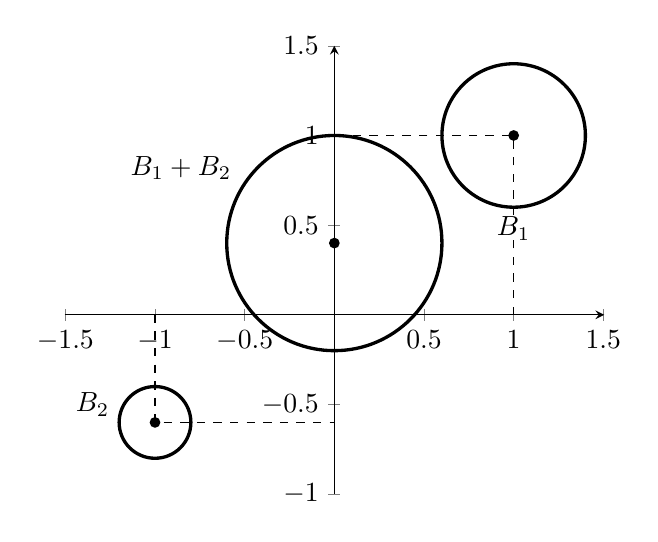
\begin{tikzpicture}
            \begin{axis}
                [axis lines = center,
                axis equal,
                trig format plots=rad,
                xmin=-1.5, xmax=1.5, ymin=-1, ymax=1.5,
                legend pos = outer north east]
                \draw [very thick] (1,1) circle (0.4);
                \draw [very thick] (-1,-0.6) circle (0.2);
                \draw [very thick] (0,0.4) circle(0.6);
                \node [below] at (1,0.6) {$B_1$};
                \node [left] at (-1.2,-0.5) {$B_2$};
                \node [above left] at (-0.52,0.7) {$B_1 + B_2$};
                \draw [dashed] (1,0) -- (1,1) -- (0,1);
                \draw [dashed] (-1,0) -- (-1,-0.6) -- (0,-0.6);
                \fill (1,1) circle (0.03);
                \fill (-1,-0.6) circle (0.03);
                \fill (0,0.4) circle (0.03);
            \end{axis}
        \end{tikzpicture}
    \end{center}
    
\end{example}
\begin{definition}
    Нехай $W(t)$ --- функція з дійсним аргументом, значеннями якої
    є компактні підмножини $\R^n$ (\emph{багатозначне відображення}).
    \emph{Інтегралом} за проміжком $[a;b]$ від неї називається множина
    $\intl_a^b W(t) dt$, яку можна розуміти в сенсі ріманової суми
    $\underset{n\to\infty}{\lim} \suml_{i=0}^n \Delta t_i\cdot W(t_i^*)$,
    де $\l\{\Delta t_i\r\}_{i=1}^n$ --- довжини відрізків, на які розбивається $[a;b]$, $t_i^* \in \Delta t_i$ ---
    деякі точки з цих відрізків, а сума розуміється в сенсі суми множин за Мінковським.
\end{definition}
\begin{example}\label{ball_intergral}
    Нехай $W(t) = B_t(0)$, $[a;b] = [0; T]$. Знайдемо 
    $\intl_0^T W(t) dt$.
    $\suml_{i=0}^n \Delta t_i\cdot W(t_i^*) = \suml_{i=0}^n \Delta t_i\cdot B_{t_i^*}(0) = 
    \suml_{i=0}^n B_{t_i^* \Delta t_i}(0) = B_{\suml_{i=0}^n t_i^* \Delta t_i} (0)$ --- це
    куля з центром в $0$ та радіусом $\suml_{i=0}^n t_i^* \Delta t_i$. Вираз для радіуса
    є інтегральною сумою для $\intl_0^t t dt = \frac{T^2}{2}$, тому
    $\intl_0^T B_t(0) dt = B_{\frac{T^2}{2}} (0)$.
\end{example}
Нехай у грі (\ref{lin_game}) виконуються дві умови:
\begin{enumerate}
    \item Для всіх $t>0$: $W(t) = \pi e^{At}U \setdif \pi e^{At}V \neq \varnothing$.
    \item Існує такий момент часу $T_0$, що $\pi e^{AT_0}z_0 \in \intl_0^T W(T_0 - s)ds$.
\end{enumerate}

Можна довести (див. \cite{4}), що в разі виконання цих умов переслідувач наздожене утікача.
Пояснення цього наводиться в \cite{3}. Розв'язок задачі Коші та його образ під дією $\pi$ у (\ref{lin_game}) мають вигляд
\begin{gather}
    z(t) = e^{A t} z_0 + \intl_0^t e^{A(t-s)} (- u(s) + v(s)) ds
\end{gather}
\begin{gather}\label{4_3}
    \pi z(t) =  \pi e^{A t} z_0 + \intl_0^t \pi e^{A(t-s)} (- u(s) + v(s)) ds
\end{gather}
За умовою 2 існує $w(T_0, s) \in W(T_0-s)$ такий, що $\pi e^{AT_0}z_0 = \intl_0^{T_0} w(T_0, s) ds$. Переслідувач має обирати своє керування
$\widehat{u}(s)$ як розв'язок рівняння
\begin{gather*}
    \pi e^{A (T_0-s)} u(s) - \pi e^{A (T_0-s)} v(s) = w(T_0, s) 
\end{gather*}
Існування розв'язку гарантується умовою 1. Якщо підставити знайдене $\widehat{u}(s)$ в (\ref{4_3}),
отримаємо 
$
    \pi z(T_0) = \pi e^{A T_0} z_0 - \intl_0^t w(T_0, s) ds = 0
$, що означає, що в момент $T_0$ переслідувач наздожене утікача.

В \cite{3} пропонується \emph{алгоритм застосування методу Понтрягіна:}
\begin{enumerate}
    \item Знайти множину $W(t) = \pi e^{At}U \setdif \pi e^{At}V$.
    \item Знайти множину $\Omega(t) = \intl_0^t W(s)ds$.
    \item Знайти $T_0$, для якого $\pi e^{A T_0} z_0 \in \Omega(T_0)$.
    \item Знайти функцію $w(t) \in W(t)$ таку, що $\pi e^{A T_0} z_0 = \intl_0^{T_0} w(s) ds$.
    \item Знайти керування $u(t)$ як розв'язок $\pi e^{A (T_0-s)} u(s) - \pi e^{A (T_0-s)} v(s) = w(T_0 - s) $ при заданому керуванні $v(t) \in V$.
    \item Знайти розв'язок задачі Коші $\d{z} = Az - u(t) + v(t), \; z(0) = z_0$ на відрізку $[0; T_0]$.
\end{enumerate}

\begin{example}(\cite{4})\label{ex_4_3}
    Нехай рух гравців в $\R^n$, $n\geq 2$, описується системою
    \begin{gather*}
        \begin{cases}
            \dd{x} + \alpha \d{x} = a, & \norm{a} \leq \rho \\
            \dd{y} + \beta \d{y} = b, & \norm{b} \leq \sigma
        \end{cases}
    \end{gather*}
    де $\alpha, \beta, \rho, \sigma$ --- додатні числа. Переслідувач наздоганяє утікача, якщо $x=y$.
    Ця системи описує рух точки одиничної маси під дією сили-керування з урахуванням тертя,
    що лінійно залежить від швидкості.
    Перейдемо до системи диференціальних рівнянь першого порядку за допомогою замін $z^1 = x - y$, $z^2 = \d{x}$, $z^3 = \d{y}$:
    \begin{gather*}
        \begin{cases}
            \d{z}^1 = z^2 - z^3 \\
            \d{z}^2 = -\alpha z^2 + a \\
            \d{z}^3 = -\beta z^3 + b
        \end{cases}
    \end{gather*}
    Керування $u$ та $v$ задаються формулами $u = (0, -a, 0)^T$, $v = (0, 0, b)^T$, тому
    $U = \l\{(0, -a, 0)^T : \norm{a} \leq \rho \r\}$, $V = \l\{(0, 0, b)^T : \norm{b} \leq \sigma \r\}$.
    Оператор $\pi$ задано як $\pi: (z^1, z^2, z^3)^T \mapsto (z^1, 0, 0)^T$, а матриця $A$
    дорівнює $\begin{pmatrix}
        0 & 1 & -1 \\
        0 & -\alpha & 0 \\
        0 & 0 & -\beta
    \end{pmatrix}$. Знайдемо $e^{A t}$ (за допомогою перетворення Лапласа):
    \begin{gather*}
        e^{At} = \Lap{(pI - A)^{-1}} \Leftrightarrow (pI - A)^{-1} = \LapInv{e^{At}} \\
        pI - A = \begin{pmatrix}
            p & -1 & 1 \\
            0 & p+\alpha & 0 \\
            0 & 0 & p + \beta \\
        \end{pmatrix} \\
        (pI - A)^{-1} = \frac{1}{p(p+\alpha)(p+\beta)}\begin{pmatrix}
            (p+\alpha)(p+\beta) & (p+\beta) & -(p+\alpha) \\
            0 & p(p+\beta) & 0 \\
            0 & 0 & p(p+\alpha)
        \end{pmatrix} = \\ =
        \begin{pmatrix}
            \frac{1}{p} & \frac{1}{p(p+\alpha)} & - \frac{1}{p(p+\beta)} \\
            0 & \frac{1}{p+\alpha} & 0 \\
            0 & 0 & \frac{1}{p+\beta}
        \end{pmatrix} \Rightarrow
        e^{At} = \begin{pmatrix}
            1 & \frac{1 - e^{-\alpha t}}{\alpha} & -\frac{1 - e^{-\beta t}}{\beta} \\
            0 & e^{-\alpha t} & 0 \\
            0 & 0 & e^{-\beta t}
        \end{pmatrix}
    \end{gather*}
    Тепер можна записати $\pi e^{At}(z^1, z^2, z^3) = z^1 + \frac{1 - e^{-\alpha t}}{\alpha} z^2 - \frac{1 - e^{-\beta t}}{\beta}z^3$, звідки
    \begin{gather*}
        \pi e^{At} U = \l\{\frac{1 - e^{-\alpha t}}{\alpha} \cdot (-a) : \norm{a} \leq \rho\r\} \\ 
        \pi e^{At} V = \l\{-\frac{1 - e^{-\beta t}}{\beta} \cdot b : \norm{b} \leq \sigma\r\}
    \end{gather*}
    Отже, $\pi e^{At} U$ --- куля з радіусом $\frac{1 - e^{-\alpha t}}{\alpha}\rho$ і центром в нулі,
    а $\pi e^{At} V$ --- куля з радіусом $\frac{1 - e^{-\beta t}}{\beta}\sigma$ і центром в нулі, тому
    $W(t) = \pi e^{At}U \setdif \pi e^{At}V$ --- куля з радіусом 
    $\frac{1 - e^{-\alpha t}}{\alpha}\rho - \frac{1 - e^{-\beta t}}{\beta}\sigma$ і центром теж в нулі.
    Радіус $W(t)$ буде додатнім при $\rho > \sigma$ та $\frac{\rho}{\alpha} > \frac{\sigma}{\beta}$.
    Аналогічно прикладу \ref{ball_intergral}, $\Omega(t) = \intl_0^t W(s) ds$ буде кулею
    з радіусом
    \begin{gather*}
        \intl_0^t \left(\frac{1 - e^{-\alpha st}}{\alpha}\rho - \frac{1 - e^{-\beta s}}{\beta} \sigma\right) ds = 
        \rho \intl_0^t \frac{1 - e^{-\alpha st}}{\alpha} ds - \sigma \intl_0^t \frac{1 - e^{-\beta s}}{\beta} ds =
    \end{gather*}
    \begin{gather*}
        = \frac{\rho}{\alpha^2}\l(\alpha t + e^{-\alpha t} - 1\r) - 
        \frac{\sigma}{\beta^2}\l(\beta t + e^{-\beta t} - 1\r)
    \end{gather*}
    Далі необхідно знайти таке (найменше) значення $T_0$, для якого точка $\pi e^{A T_0}(z^1_0, z^2_0, z^3_0)$ належить
    $\Omega(T_0)$. З геометричних міркувань це буде найменший корінь рівняння
    \begin{gather*}
        \l( \frac{\rho}{\alpha^2}\l(\alpha t + e^{-\alpha t} - 1\r) - 
        \frac{\sigma}{\beta^2}\l(\beta t + e^{-\beta t} - 1\r)\r)^2 = \norm{\pi e^{A t} z_0}^2
    \end{gather*}
    
    Наступний крок будемо проводити на конкретному прикладі. Нехай гра відбувається на площині
    з початковими умовами $x(0) = \begin{pmatrix}
        3 \\ 2
    \end{pmatrix}, \d{x}(0) = \begin{pmatrix}
        1 \\ 1
    \end{pmatrix}, y(0) = \begin{pmatrix}
        1 \\ 0
    \end{pmatrix}, \d{y}(0) = \begin{pmatrix}
        0 \\ 1
    \end{pmatrix}$. Чисельно можна знайти $T_0 \approx 3.715$.
\end{example}
\begin{example}
    Розглянемо тепер гру з простим рухом:
    \begin{gather*}
        \begin{cases}
            \d{x} = u, & \norm{u} \leq \alpha \\
            \d{y} = v, & \norm{v} \leq \beta 
        \end{cases}
    \end{gather*}
    Зробимо заміну $z = x - y$: $\d{z} = u - v = -(-u) + (-v)$.
    переслідування закінчується, коли $z = x - y = 0$.
    В такому випадку оператор $\pi$ є тотожнім, матриця $A$ --- нульовою,
    тому й композиція $\pi e^{At} = I$ --- теж тотожній оператор.
    $U = B_{\alpha}(0)$, $V = B_{\beta}(0)$ --- кулі з центрами в $0$ та з радіусами
    $\alpha$ та $\beta$ відповідно. Таким чином, $W(t) = 
    \pi e^{At} U \setdif \pi e^{A t} V = U \setdif V = B_{\alpha - \beta}(0)$,
    при $\alpha \geq \beta$ ця множина є непорожньою.
    $\Omega(t) = \intl_0^t W(s)ds = B_{t(\alpha - \beta)}(0)$, тому
    \begin{gather*}
        \pi e^{AT_0} z_0 \in \Omega(T_0) \Leftrightarrow z_0 \in B_{T_0(\alpha - \beta)}(0) \Leftrightarrow
        \norm{z_0} = T_0(\alpha - \beta) \Leftrightarrow T_0 = \frac{\norm{z_0}}{\alpha - \beta}
    \end{gather*}
    Зауважимо, що такий само час було отримано у \ref{sec_3_2} іншими міркуваннями.
    Тепер знайдемо $w(t) \in W(t)$, для якої $\pi e^{A T_0} z_0 = \intl_0^{T_0} w(s)ds$:
    \begin{gather*}
        \pi e^{A T_0} z_0 = z_0 = \intl_0^{\frac{\norm{z_0}}{\alpha - \beta}} w(s) ds \Rightarrow
        w(s) \equiv (\alpha - \beta)\cdot \frac{z_0}{\norm{z_0}}
    \end{gather*}
    Для заданого керування утікача $v(t)$ знайдемо керування переслідувача $u(t)$:
    \begin{gather*}
        \pi e^{A (T_0-s)} u(s) - \pi e^{A (T_0-s)} v(s) = w(T_0 - s) \\
        u(s) - v(s) = (\alpha - \beta)\cdot \frac{z_0}{\norm{z_0}} \Leftrightarrow
        u(s) = v(s) + (\alpha - \beta)\cdot \frac{z_0}{\norm{z_0}}
    \end{gather*}
    Таким чином, можемо розв'язати задачу Коші
    \begin{gather*}
        \begin{cases}
            \d{z} = -u + v = (\beta - \alpha)\cdot \frac{z_0}{\norm{z_0}} \\
            z(0) = z_0
        \end{cases} \Rightarrow
        z(t) = (\beta - \alpha)\cdot \frac{z_0}{\norm{z_0}} t + z_0 \Leftrightarrow \\ \Leftrightarrow
        x(t) - y(t) = (\beta - \alpha)\cdot \frac{x_0 - y_0}{\norm{x_0 - y_0}} t + (x_0 - y_0)
    \end{gather*}
\end{example}

\section{Метод розв'язуючих функцій}
%Цей метод належить А.О. Чикрію та детально досліджений у \cite{6}.
%Розглядається не просто 